
\chapter{Cấu tạo và tính chất của thấu kính mỏng}
\section{Lý thuyết trọng tâm}
\subsection{Thấu kính. Phân loại thấu kính}
Thấu kính là một khối trong suốt (thủy tinh, nhựa, ...) giới hạn bởi hai mặt cong hoặc một mặt cong và một mặt phẳng.

Có hai loại thấu kính:

		
	\begin{itemize}
		\item Thấu kính lồi (có rìa mỏng).
		\item Thấu kính lõm (có rìa dày).
			\end{itemize}
\begin{center}
	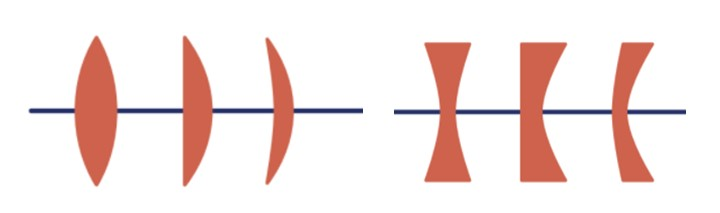
\includegraphics[scale=0.5]{../figs/VN11-PH-38-L-026-1-h4.jpg}
\end{center}
Trong không khí, thấu kính lồi là \textit{thấu kính hội tụ}, thấu kính lõm là \textit{thấu kính phân kì}.
	\subsection{Khảo sát thấu kính hội tụ và phân kỳ}
	
\subsubsection{Quang tâm. Trục chính. Trục phụ}
\begin{itemize}
	\item O là điểm chính giữa thấu kính. Và được gọi là quang tâm của thấu kính.
	\item Đường thẳng đi qua quang tâm O và vuông góc với mặt thấu kính là trục chính của thấu kính.
	\item Các đường thẳng khác qua quang tâm O nhưng không vuông góc với mặt kính là trục phụ.
	\end{itemize}
\begin{center}
	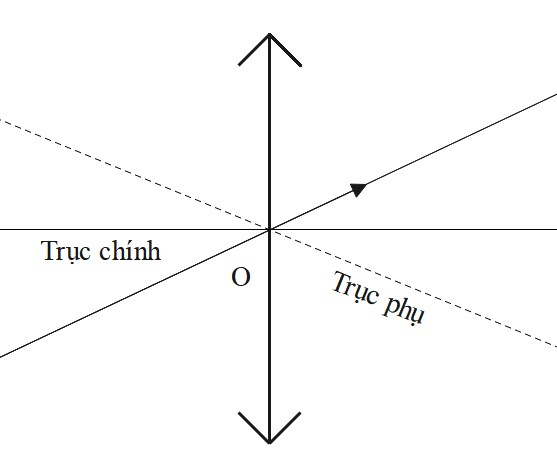
\includegraphics[scale=0.5]{../figs/VN11-PH-38-L-026-1-h7.jpg}
\end{center}

\subsubsection{Tiểu điểm. Tiêu diện}
Trên mỗi trục có một tiêu điểm ảnh:
\begin{itemize}
	\item Tiêu điểm ảnh chính, kí hiệu là F'. 
	\item Tiêu điểm ảnh phụ, kí hiệu là $\text{F'}_\text{n}\ (n=1,2,3,...)$.
\end{itemize}

Tương tự, trên mỗi trục cũng có một tiêu điểm vật:
\begin{itemize}
	\item Tiêu điểm vật chính, kí hiệu là F.
	\item Tiêu điểm vật phụ, kí hiệu là $\text{F'}_{\text{n}}\ (n=1,2,3,...)$.
\end{itemize}
\begin{center}
	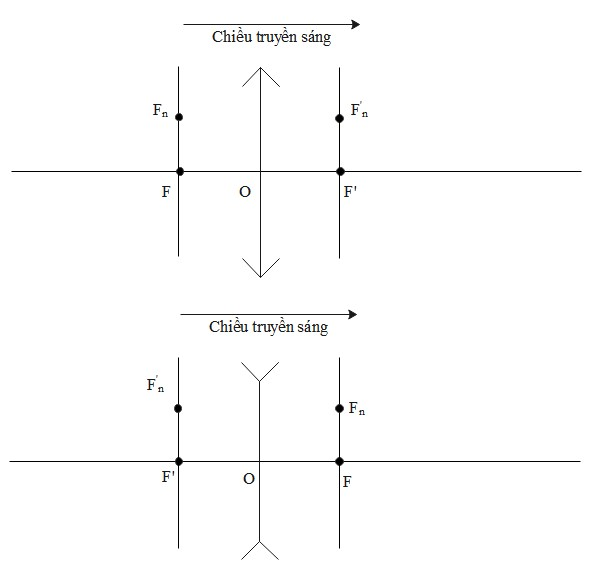
\includegraphics[scale=0.8]{../figs/VN11-PH-38-L-026-1-h18.jpg}
\end{center}



Tiêu điểm ảnh và tiêu điểm vật trên một trục nằm đối xứng với nhau qua quang tâm.  

Tập hợp tất cả các tiêu điểm tạo thành tiêu diện. Có thể coi tiêu diện là mặt phẳng vuông góc với trục chính và qua tiêu điểm chính. Mỗi thấu kính có hai tiêu diện: tiêu diện ảnh và tiêu diện vật. 

	
\subsubsection{Tiêu cự. Độ tụ}
Tiêu cự của thấu kính được định nghĩa như sau:
\begin{equation}
f=\overline{\text{OF'}},
\end{equation}
trong đó:
\begin{itemize}
	\item $f$ là tiêu cự của thấu kính, 
	\item $\overline{\text{OF'}}$ là giá trị đại số của khoảng cách từ quang tâm O đến các tiêu điểm chính.
\end{itemize}
\textbf{Quy ước}: Thấu kính hội tụ thì tiêu cự $f>0$, thấu kính phân kỳ thì tiêu cự $f<0$.

Độ tụ của thấu kính được tính theo công thức sau:
\begin{equation}
D=\dfrac{1}{f},
\end{equation}
trong đó:
\begin{itemize}
	\item $D$ là độ tụ của thấu kính, đơn vị là điốp (dp). 
	\item $f$ là tiêu cự của thấu kính, đơn vị là mét (m).
\end{itemize}
Thấu kính có khả năng hội tụ chùm tia sáng càng mạnh khi độ tụ $D$ càng lớn, tức $f$ càng nhỏ. Tương tự, thấu kính có khả năng phân kỳ chùm tia sáng càng mạnh khi độ tụ $D$ càng âm, tức $f$ càng gần 0.
\section{Bài tập }
%\begin{dang}{Các tính chất của thấu kính}
%\end{dang}

\viduii{1}{

 Chọn phát biểu \textbf{không đúng}
\begin{mcq}
	\item Thấu kính hội tụ có tiêu cự $f>0$.
	\item Thấu kính phân kỳ có tiêu cự $f>0$.
	\item Các đường thẳng khác qua quang tâm O nhưng không vuông góc với mặt kính là trục phụ.
	\item Tiêu điểm ảnh và tiêu điểm vật trên một trục nằm đối xứng với nhau qua quang tâm.
\end{mcq}
}
{
\begin{center}
	\textbf{Hướng dẫn giải:}
\end{center}

{Theo quy ước, thấu kính phân kỳ có tiêu cự $f<0$.
	
	\textbf{Đáp án: B.}
}
}
\viduii{1}{
Chọn phát biểu \textbf{không đúng}.
\begin{mcq}
	\item Trong không khí, thấu kính lồi là \textit{thấu kính hội tụ}, thấu kính lõm là \textit{thấu kính phân kì}.
	\item Thấu kính là một khối trong suốt (thủy tinh, nhựa, ...) giới hạn bởi hai mặt cong hoặc một mặt cong và một mặt phẳng.
	\item Có thể coi tiêu diện là mặt phẳng vuông góc với trục chính và qua tiêu điểm chính.
	\item Thấu kính có khả năng hội tụ chùm tia sáng càng mạnh khi $f$ càng lớn.
\end{mcq}}
{

\begin{center}
	\textbf{Hướng dẫn giải:}
\end{center}

{Thấu kính có khả năng hội tụ chùm tia sáng càng mạnh khi $f$ càng nhỏ.
\textbf{	Đáp án: D.}
}
}
\viduii{1}{
Chọn phát biểu đúng.
\begin{mcq}
	\item Tiêu điểm ảnh và tiêu điểm vật trên một trục nhưng không đối xứng với nhau qua quang tâm. 
	\item Công thức tính độ tụ là $D=\dfrac{1}{f^2}$.
	\item Các đường thẳng khác qua quang tâm O nhưng không vuông góc với mặt kính là trục phụ. 
	\item Thấu kính phân kỳ thì tiêu cự $f>0$. 
\end{mcq}}
{

\begin{center}
	\textbf{\textbf{Hướng dẫn giải:}}
\end{center}

{ Tiêu điểm ảnh và tiêu điểm vật trên một trục và đối xứng với nhau qua quang tâm. Do đó, câu A không đúng.
	
	Công thức tính độ tụ là $D=\dfrac{1}{f}$. Do đó, câu B không đúng.
	
	Thấu kính phân kỳ thì tiêu cự $f<0$. Do đó, câu D không đúng.
	
	Các đường thẳng khác qua quang tâm O nhưng không vuông góc với mặt kính là trục phụ. Do đó, câu C đúng.
		
	\textbf{Đáp án: C.}
}
}
